\section{Approach}

\begin{figure}[t!]
\centering
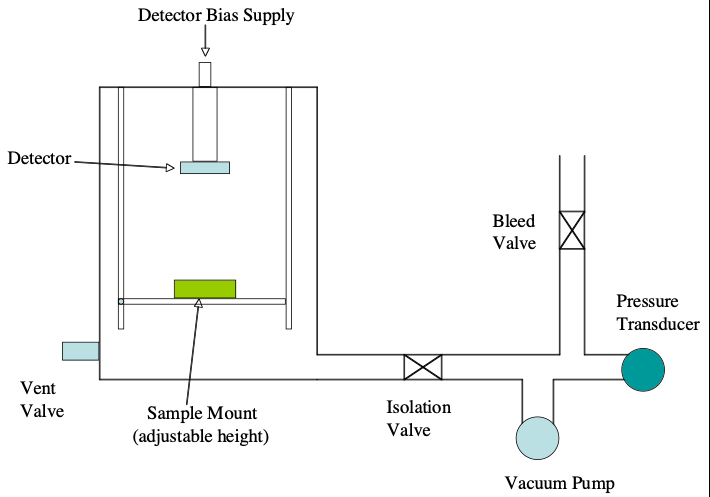
\includegraphics[scale=0.7]{alpha_setup.png}
\caption{Schematic diagram of the experimental setup for calculating the range of Am-241 $\alpha$ particles. The detector is placed a fixed distance away from the source and enclosed in a pressure chamber. The stopping medium can be varied by changing its pressure in the chamber.}
\label{fig:alpha-setup}
\end{figure}

\begin{figure}
\centering
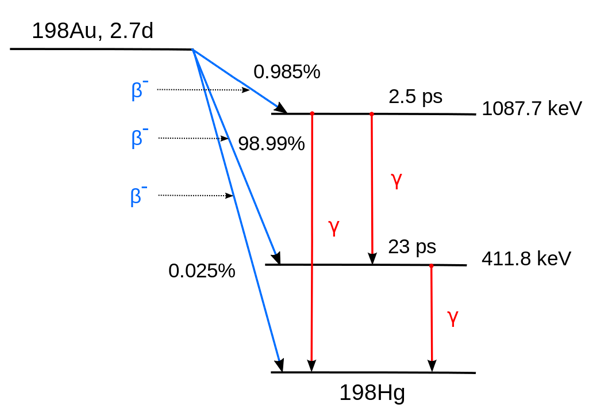
\includegraphics[scale=0.7]{au198.png}
\caption{Au-198 decay scheme. This decay has one very intense $\gamma$ emission at 411.8 keV. This can be used to measure a mass attenuation coefficient by measuring the photopeak magnitude/intensity at different shielding thicknesses.}
\label{fig:au198}
\end{figure}

\begin{figure}
\centering
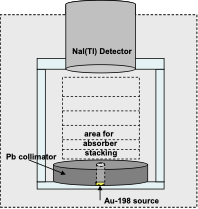
\includegraphics[scale=0.7]{gamma_setup.png}
\caption{Schematic diagram of the experimental setup for calculating the mass attenuation coefficients for lead and aluminum. This probes their performance at shielding $\gamma$ radiation emitted from an Au-198 source. Space is left between the detector and the source so that varying thicknesses of shielding material can be applied. The source is collimated with a lead disk that can be plugged to block source radiation.}
\label{fig:gamma-setup}
\end{figure}

To experimentally measure a stopping range of $\alpha$ particles, a controlled experimental setup was created that can very the amount of stopping medium between the radioactive source and the detector. A schematic diagram of the setup can be seen in Fig. \ref{fig:alpha-setup}. The sample used here is an Am-241 source that emits $\alpha$ particles at an energy of 5.486 MeV. Radiation from this source is then detected using a Silicon detector. To probe the distance the radiation can travel, the stopping medium is controlled by adjusting the pressure in the chamber. A digital voltmeter is used as a pressure sensor readout. While this reads a voltage value, the pressure in the chamber can be inferred since both pressure and voltage will change linearly and proportionally. Recording the voltage at atmospheric pressure provides a reference point to calculate the chamber pressure at other voltage readings. Finally, using a multi-channel analyzer (MCA), an energy spectrum can be recorded for several pressure values. Measuring the net counts of the $\alpha$ peak (5.486 MeV) then provides a stopping power relationship that can be used to calculate a range.

To measure mass attenuation coefficients for lead and aluminum, a Sodium Iodide (NaI) Detector is used. This is fitted into apparatus where an Au-198 source can be fitted. The decay scheme for Au-198 can be seen in Fig. \ref{fig:au198}. While there are three possible $\gamma$ emissions from this decay scheme, the high intensity 411.8 keV peak can be used to measure radiation intensity. The experimental setup is illustrated in Fig. \ref{fig:gamma-setup}. This source is collimated using a lead collimating disk. Background radiation can be measured by plugging the collimator with a lead plug. There is then space between the source and the detector to stack shielding material. Layers of lead or aluminum can be placed in this region and the radiation intensity (or count-rate) can be measured for varying thicknesses. This can then be fitted to characteristic exponential decay and a mass attenuation coefficient can be determined for each material.

For each experimental setup, a traditional data acquisition system is used. Bias voltage is applied to the detector. A combination of a preamplifier and amplifier are used to boost the initial detector signal. An oscilloscope can be used for diagnostics. This output is fed to a multi-channel analyzer (MCA) that can bin signatures relative to the voltage detected. For the $\gamma$ setup, a single-channel analyzer (SCA) and counter were also used to measure the count-rate of a single peak channel.
